\documentclass[11pt]{book}
\usepackage{caption,graphicx}
\usepackage{float}
\usepackage{indentfirst}
\usepackage{float} 
\parskip 5pt    
\usepackage[margin=1in]{geometry}
\setcounter{section}{0}
\renewcommand{\thesection}{\arabic{section}}
\usepackage{amssymb}
\usepackage{enumitem}
\usepackage{setspace}
\linespread{1.0}
\begin{document}
\renewcommand{\labelitemi}{$\textendash$}
\renewcommand{\labelitemii}{{\tiny$\blacksquare$}}

\title{Bachelor's Thesis: Implementing Security in IoT Gateway in Legacy Devices for Telemedicine Applications. A comparison between Lightweight IPsec and CoAP}
\author{Perla Rocío Ramírez Sanabria}
\date{\small{\today}}
\maketitle

\setcounter{tocdepth}{2}
\tableofcontents
\break

\chapter{Introduction}
\chapter{IoT: Internet of Things}
\section{Definition}
\section{Applications}
\subsection{Application: Telemedicine}
\section{IoT Gateway}
\chapter{IPsec: Internet Protocol Security}
\section{Definition}
IPsec results from the abbreviation of Internet Protocol Security. This protocol provides a framework of open standards to ensure secure communications over IPv4 or IPv6, authenticating and encrypting each packet, thus ensuring communications at the network level and at all higher levels. Being optional for IPv4 and mandatory for IPv6.\\
IPsec can be implemented in several ways such as:
\begin{itemize}
\item Site-to-Site Connections (Networks Interconnection)
\item Host-to-Host Connections
\item Host-to-Site Connections (Remote Access)
\end{itemize}
And there exist several benefits about implementing IPsec:
\begin{itemize}
\item Transparent for protocols such as TPC and UPD as well for users and applications.
\item It improves the security provided by other mechanisms such as SSL, TLS or SSH, operating all these at level 4 or higher.
\item Possibility of integrating it into a perimeter security device.
\end{itemize}


\section{Modes}
IPsec operates in two possible modes, transport or tunnel which are going to be discussed in the following subsections.
\subsection{Transport}
When working with this mode the original IP packet is modified by inserting an additional header between the network and transport layer only protecting the information coming from the transport layer. 
\begin{figure}[H]
	\centering
	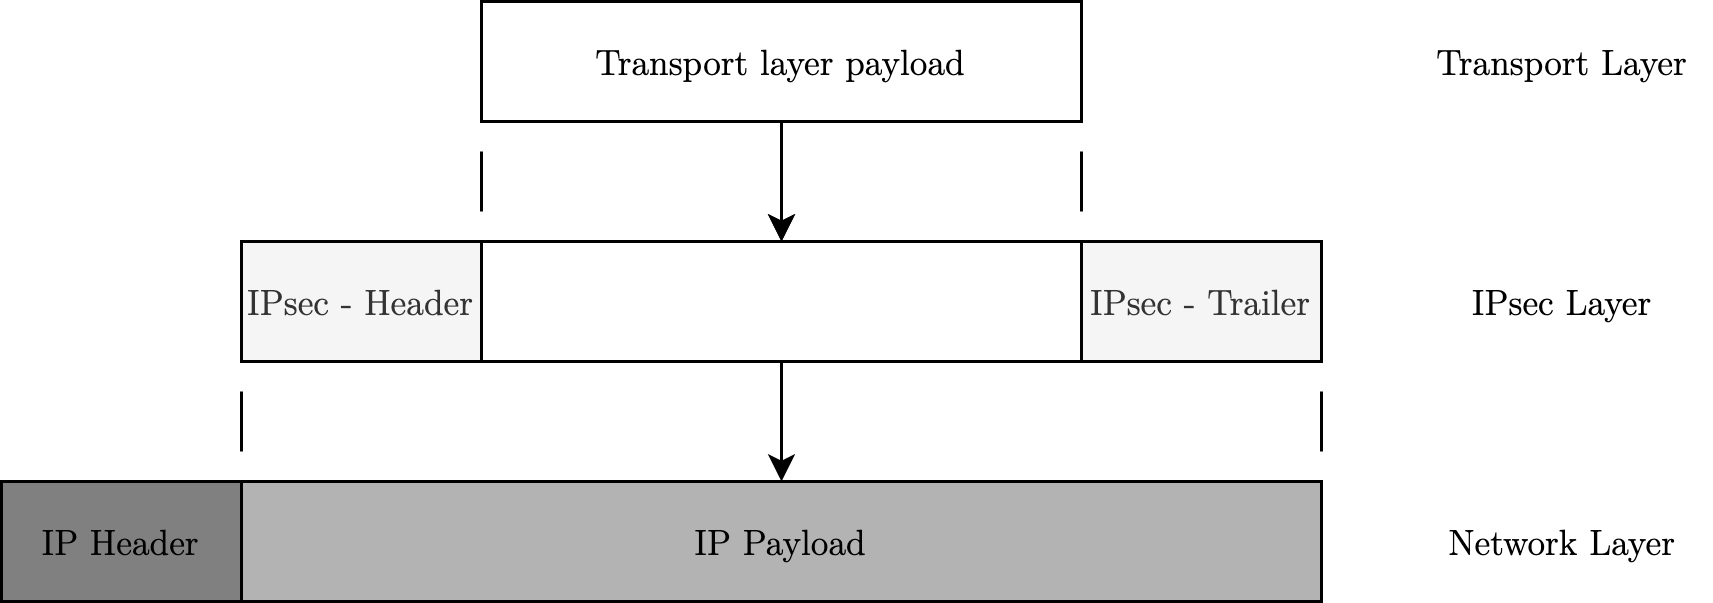
\includegraphics [scale=0.165] {transport_encapsulation.png}
	\caption{IPsec in transport mode}
\end{figure}
As it can be seen, the segment of the transport layer is encapsulated with a header and a trailer, this resulting encapsulation will be the final IP packet data field where the source and destination IP addresses are those of the two nodes that want to communicate securely.\\

\subsection{Tunnel}
When working with this mode the original IP packet is encapsulated entirely in a new IP packer, where the new IP header will have as origin and destination addresses the ends of the tunnel. Therefore, the entire packet is protected unlike when working with the transport mode. 
\begin{figure}[H]
	\centering
	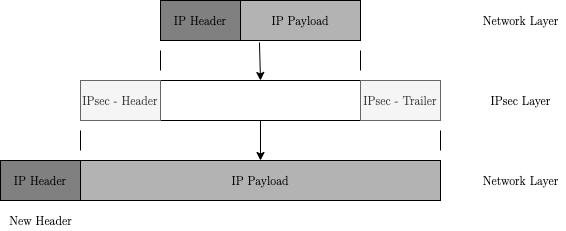
\includegraphics [scale=0.165] {tunnel_encapsulation.png}
	\caption{IPsec in tunnel mode}
\end{figure}
In tunnel mode it is the original IP packet the one being encapsulated with an IPsec header and a trailer. A new IP header is added to the resulting encapsulation, where, as already said before, the source and destination IP addresses are those at the ends of the tunnel.
\section{Components of IPsec}
\subsection{Security Protocols}
\subsubsection{AH: Authentication Header}
The AH security protocol provides authentication and integrity to the IP packets transmitted, but without encryption. This means that there is a guarantee that the data was sent by a legitimate sender and it has not been altered, but there is no guarantee for confidentiality. This will also prevent IP packets' replay and at the same time it protects immutable fields in IP header.\\
In order to protect the IP header and data against modifications, a MAC (Message Authentication Code) function is applied to the majority of the bytes of the IP datagram, except for the fields that could change such as TOS, Flags, Checksum and TTL fragments offset. The minimum requirements for this MAC function are HMAC-MD5-96 and HMAC-SHA-1-96.
\begin{figure}[H]
	\centering
	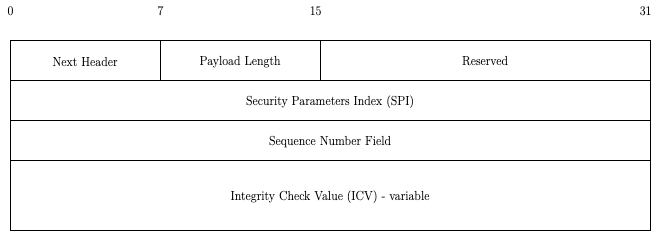
\includegraphics [scale=0.175] {ah_fields.png}
	\caption{AH fields}
\end{figure}

The AH extension contains the following fields:
\begin{itemize}
\item \textbf{Next Header:} this field is 1 byte long and it is used in order to identify the type of the next payload after the Authentication Header. The value assigned to this field will vary depending on the protocol used and it is chosen from the set of IP Protocol Number that is defined by the IANA. For example, 1 for ICMP, 6 for TCP, 17 for UDP, etc. 
\item \textbf{Payload Length:} this field is 1 byte long and it is used to specify the length of AH in multiples of 4 bytes (32 bits), excluding the first 8 bits.
\item \textbf{Reserved:} this field is 2 bytes long and it is reserver for future use. Since it is not used currently, the sender must set a value ``0" for this field and it should be ignored by the recipient. 
\item \textbf{Security Parameters Index (SPI):} this field is 4 bytes long and it is used to identify the SA (Security Association), which will be discussed later in this document. 
\item \textbf{Sequence Number:} this field is 4 bytes long and it contains a counter value for all the packets sent, this means that with every packet sent this value will increase. The sender must include even if the recipient does not activate the anti replay protection, in which case it will be ignored by the latter.
\item \textbf{Extended Sequence Number (ESN):} this field is 8 bytes long and it is used to support high-speed IPsec implementations by at the same time prolonging a SA's lifetime. This ESN must be negotiated when SA is created by the SA management protocol. This works as an extension of the already existing 4 bytes sequence number field.
\item \textbf{Integrity Check Value (ICV):} this field has a variable length and it contains the ICV, which will provide authentication and integrity checking. Its length must be an integral multiple of 32 bits for both IPv4 and IPv6. 
\end{itemize}

\break

In the following figures we can see the AH encapsulation with the two possible modes:
\begin{figure}[H]
	\centering
	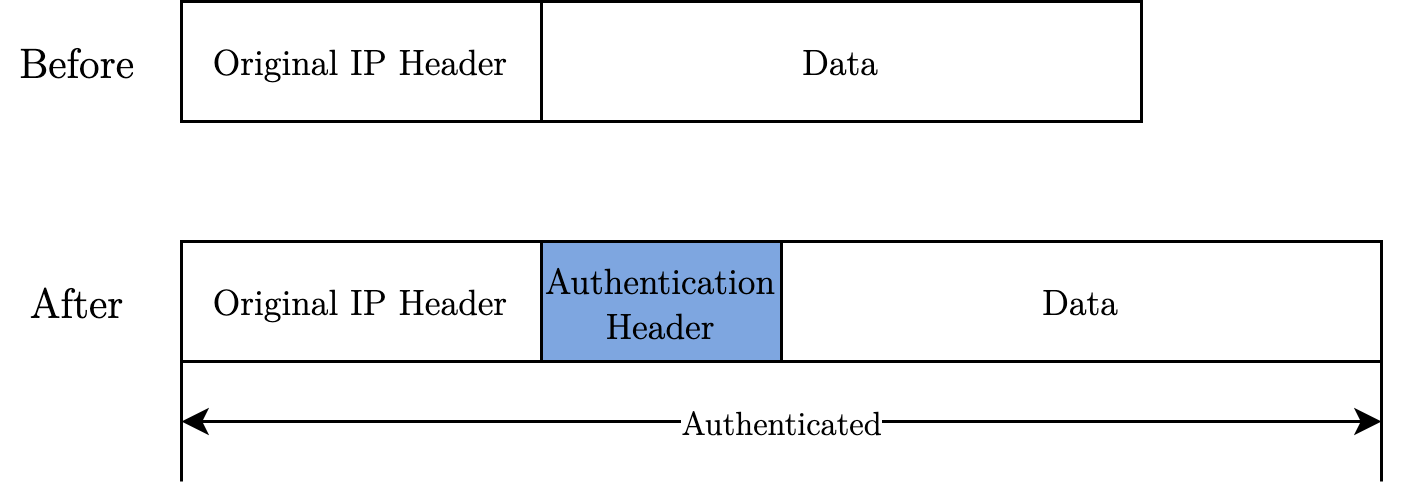
\includegraphics [scale=0.17] {ah-transport.png}
	\caption{AH Encapsulation in transport mode}
\end{figure}
\begin{figure}[H]
	\centering
	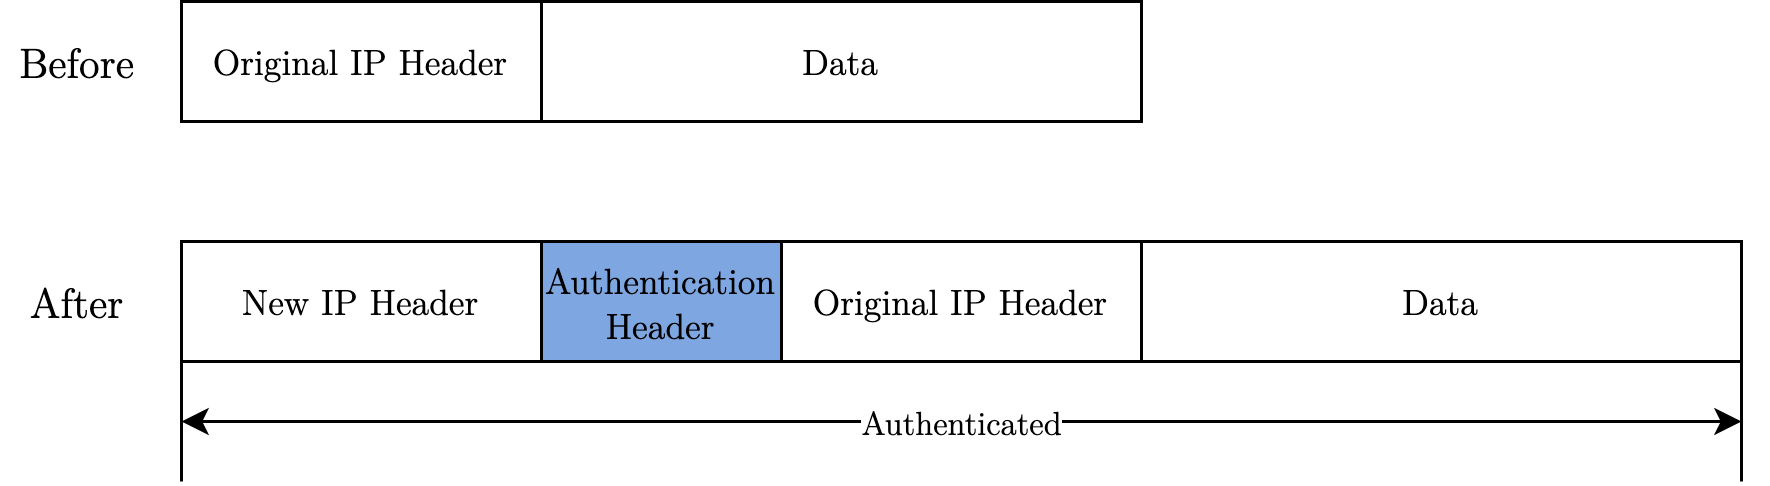
\includegraphics [scale=0.17] {ah-tunnel.png}
	\caption{AH Encapsulation in tunnel mode}
\end{figure}

\subsubsection{ESP: Encapsulating Security Payload}
The ESP security protocol provides data integrity, source authentication and confidentiality of IP packets. However, ESP does not provide integrity and authentication for the entire IP packet, which is the reason why there exist the possibility to combine it with AH.\\
It guarantees that the content cannot be examined by third parties or, if possible, that it cannot be interpreted. It will be necessary to use a key in order to encrypt the data and different encryption algorithms can be used, such as DES, 3DES, RC5, etc. \\
It is important to note that ESP does not encrypt nor authenticate the IP header fields unless they are encapsulated by ESP using the tunnel mode. 
\begin{figure}[H]
	\centering
	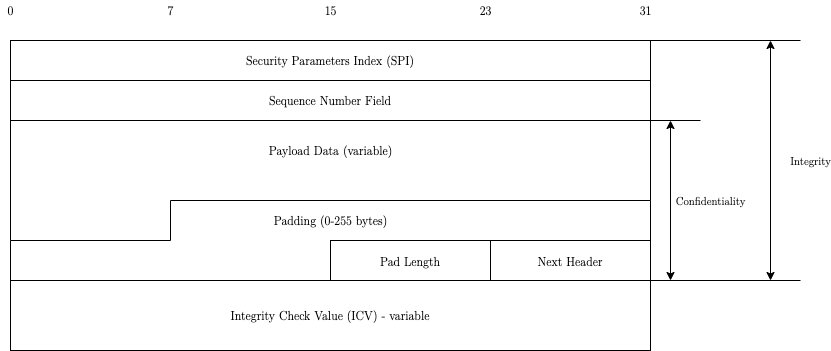
\includegraphics [scale=0.165] {esp_header.png}
	\caption{ESP fields}
\end{figure}
The ESP extension contains the following fields:
\begin{itemize}
\item \textbf{ESP Header:} 
	\begin{itemize}
	\item \textbf{Security Parameters Index (SPI):} this field is 4 bytes long and it is used to identify the SA (Security Association), which will be discussed later in this document. 
	\item \textbf{Sequence Number:} this field is 4 bytes long and it contains a counter value for all the packets sent, this means that with every packet sent this value will increase. The sender must include even if the recipient does not activate the anti replay protection, in which case it will be ignored by the latter.
	\item \textbf{Extended Sequence Number (ESN):} this field is 8 bytes long and it is used to support high-speed IPsec implementations by at the same time prolonging a SA's lifetime. This ESN must be negotiated when SA is created by the SA management protocol. This works as an extension of the already existing 4 bytes sequence number field.
\end{itemize}
\item \textbf{Payload Data:} this field has a variable length that will vary depending on the length of the data. Contains data described by the Next Header field as well as the initialisation vector for the encryption algorithm. It is the information that is actually protected by ESP.
\item \textbf{ESP Trailer:}
	\begin{itemize}
	\item \textbf{Padding:} there are two factors why this field is needed: 
		\begin{enumerate}
		\item The requirement for the plaintext to be a multiple of a certain number.
		\item The requirement for the resulting ciphertext to terminate on a 4-byte boundary.
		\end{enumerate}
	This field has a variable length that can go from 0 to 255 bytes depending on the requirements needed. 
	\item \textbf{Pad Length:} this field is 1 byte long and it is used to specify the length of the previously mentioned padding. It accepts values from 0 to 255, where a ``0" value indicates the absence of Padding bytes.
	\item \textbf{Next Header:} this field is 1 byte long and it is used in order to identify the type of the next payload after the Authentication Header. The value assigned to this field will vary depending on the protocol used and it is chosen from the set of IP Protocol Number that is defined by the IANA. For example, 1 for ICMP, 6 for TCP, 17 for UDP, etc. 
	\end{itemize}
\item \textbf{Integrity Check Value:} this field has a variable length and it is the result of the computation over the ESP header, Payload, and ESP trailer fields.
\end{itemize}
In the following figures we can see the ESP encapsulation with the two possible modes:
\begin{figure}[H]
	\centering
	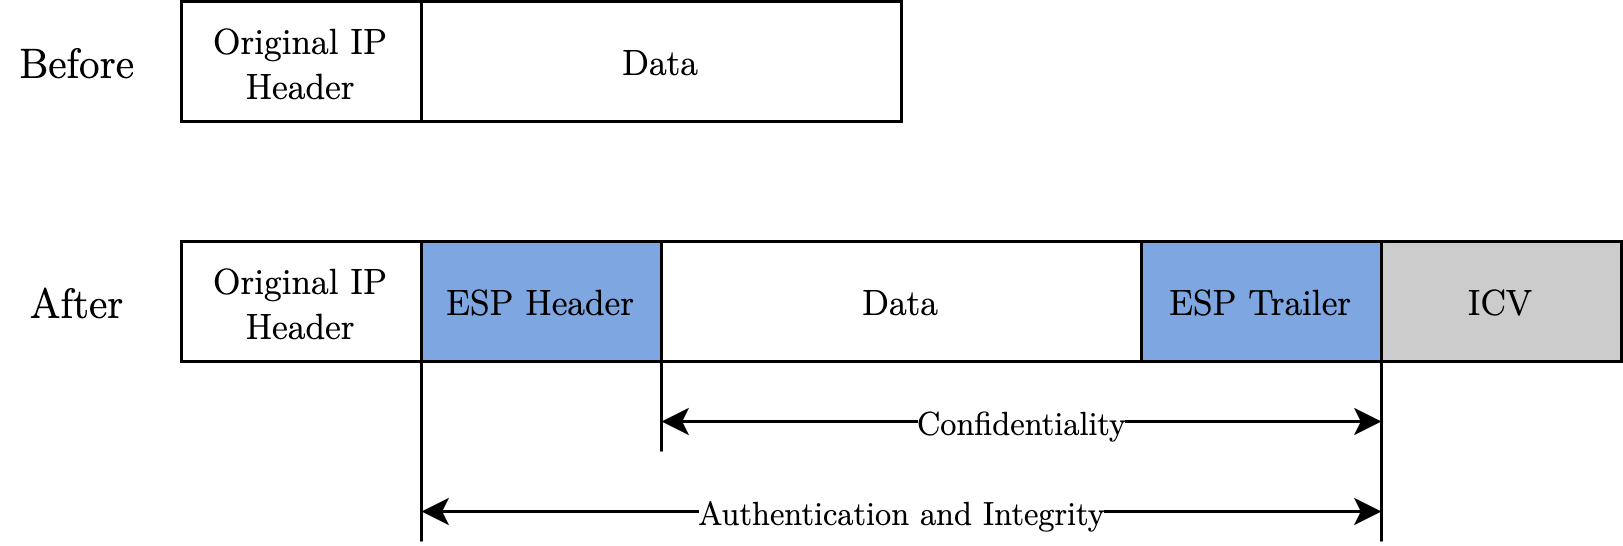
\includegraphics [scale=0.175] {esp-transport.png}
	\caption{ESP Encapsulation in transport mode}
\end{figure}
\begin{figure}[H]
	\centering
	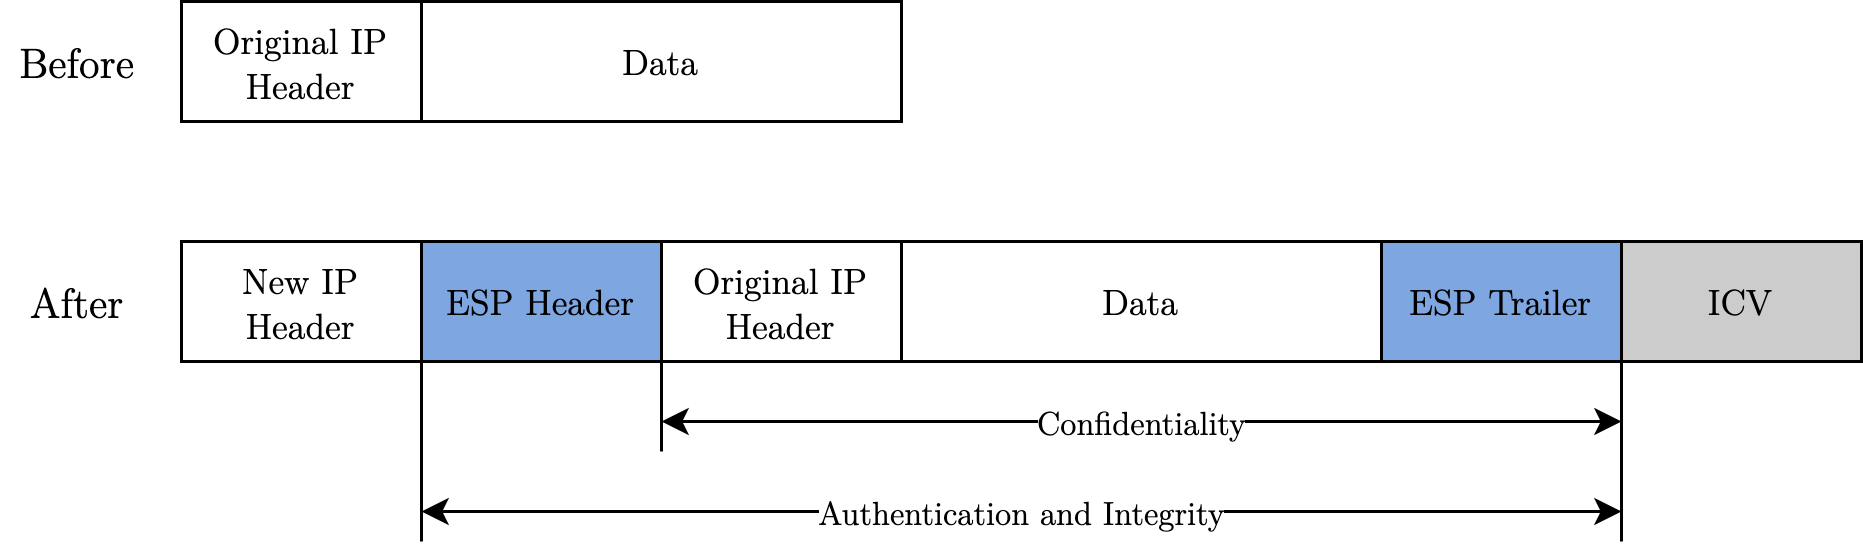
\includegraphics [scale=0.175] {esp-tunnel.png}
	\caption{ESP Encapsulation in tunnel mode}
\end{figure}


\subsubsection{ Security Associations}
An IPsec Security Association specifies the security properties for the traffic between the parties in a communication. Within these SAs the needed parameters such as encryption algorithms or keys are negotiated. These SAs are created dynamically by the Internet Key Exchange (IKE) protocol, which is going to be discussed in more detail later in the document.\\
An SA constitutes a simplex connection, which means that if the connection needs to be protected in both ways two SA's are required. Additionally, in every SA there is a possibility to use AH and ESP, but not simultaneously. Therefore, two SAs are required for each direction if both security protocols are used.\\
There are three parameters that defines an SA uniquely:
\begin{itemize}
\item Security Parameter Index (SPI)
\item Destination IP Address (DA)
\item Protocol identifier (P)
\end{itemize}
The three values previously mentioned are included in the data sent and in the Security Association Database (SAD) as we can see in the figure below:
\begin{figure}[H]
	\centering
	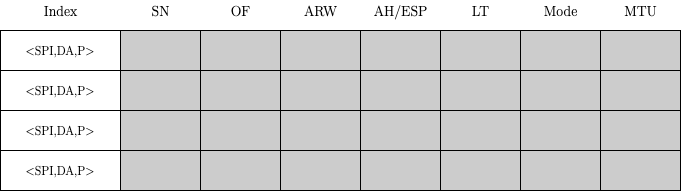
\includegraphics [scale=0.165] {sadb_table.png}
	\caption{Security Association Database}
\end{figure}
A Security Association Database (SAD) a central repository that contains all the active SAs for both inbound and outbound processes. With each entry on the database the specific parameters for each SA are defined.
\begin{itemize}
\item \textbf{SN (Sequence Number):} 32-bit value used to generate sequence numbers for the security protocols.
\item \textbf{OF (Overflow Flag)}
\item\textbf{ ARW (Anti-Replay Window):} detects inbound replayed packet.
\item \textbf{AH/ESP:} 
	\begin{itemize}
	\item AH Information: Authentication algorithm, Keys, Key lifetime, others.
	\item ESP Information:Encryption algorithm, Authentication algorithm, Keys, Key lifetime, Initialisation vectors, others.
	\end{itemize}

\item \textbf{LT (Lifetime):} specifies the lifetime for the SA.
\item \textbf{Mode:} specifies the mode, which can be transport or tunnel.
\item \textbf{MUT(Path MTU):} specifies the path MTU. 
\end{itemize}


\section{Key Management. Internet Key Exchange (IKE)}
The IKE protocol is not a part of the IPsec specification, but it is integrated with it. As it was stated before in this document, it is the one in charge to create SAs, negotiate security policies, perform key exchange and authenticate the nodes.\\
It is a hybrid protocol based on the framework defined by Internet Security Association and Key Management Protocol (ISAKMP) and two other key management protocols: Oakley and SKEME. The latter protocols define a method with a view to establish an authenticated key exchange. The tasks for these protocols are:
\begin{itemize}
\item \textbf{ISAKMP:} provides a framework for authentication and key exchange by defining the format of the messages.
\item \textbf{Oakley:} It is the protocol for determining symmetric keys, based on Diffie-Hellman, but with additional security.
\item \textbf{SKEME:} ``describes a versatile key exchange technique which provides anonymity, repudiability, and quick key refreshment" (RFC IKE)
\end{itemize}
Regarding the authentication, there two possible techniques:
\begin{itemize}
\item \textbf{Pre-Shared Key (PSK)}, from which an authentication hash is created and exchanged between the parties.
\item \textbf{RSA Signature}, a hash is signed with the private key and then exchanged  between the parties. 
\end{itemize}
It divides its activity into two phases:
\begin{itemize}
\item \textbf{PHASE 1:} Negotiation of the IKE SA to protect phase 2 and it has two possible modes: main and aggresive.
\item \textbf{PHASE 2:} Negotiation of SA for a data exchange protocol, in our case IPsec in each flow.
\end{itemize}

\break

In the following figures we can se the two phases implementing both modes for PHASE 1:
\begin{figure}[H]
	\centering
	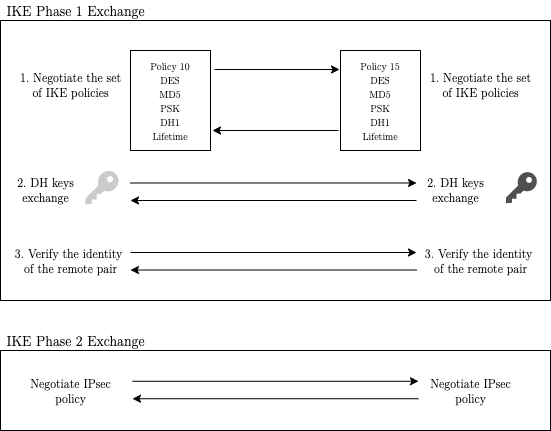
\includegraphics [scale=0.19] {main.png}
	\caption{IKE: Phase 1 and Phase 2}
\end{figure}

\begin{figure}[H]
	\centering
	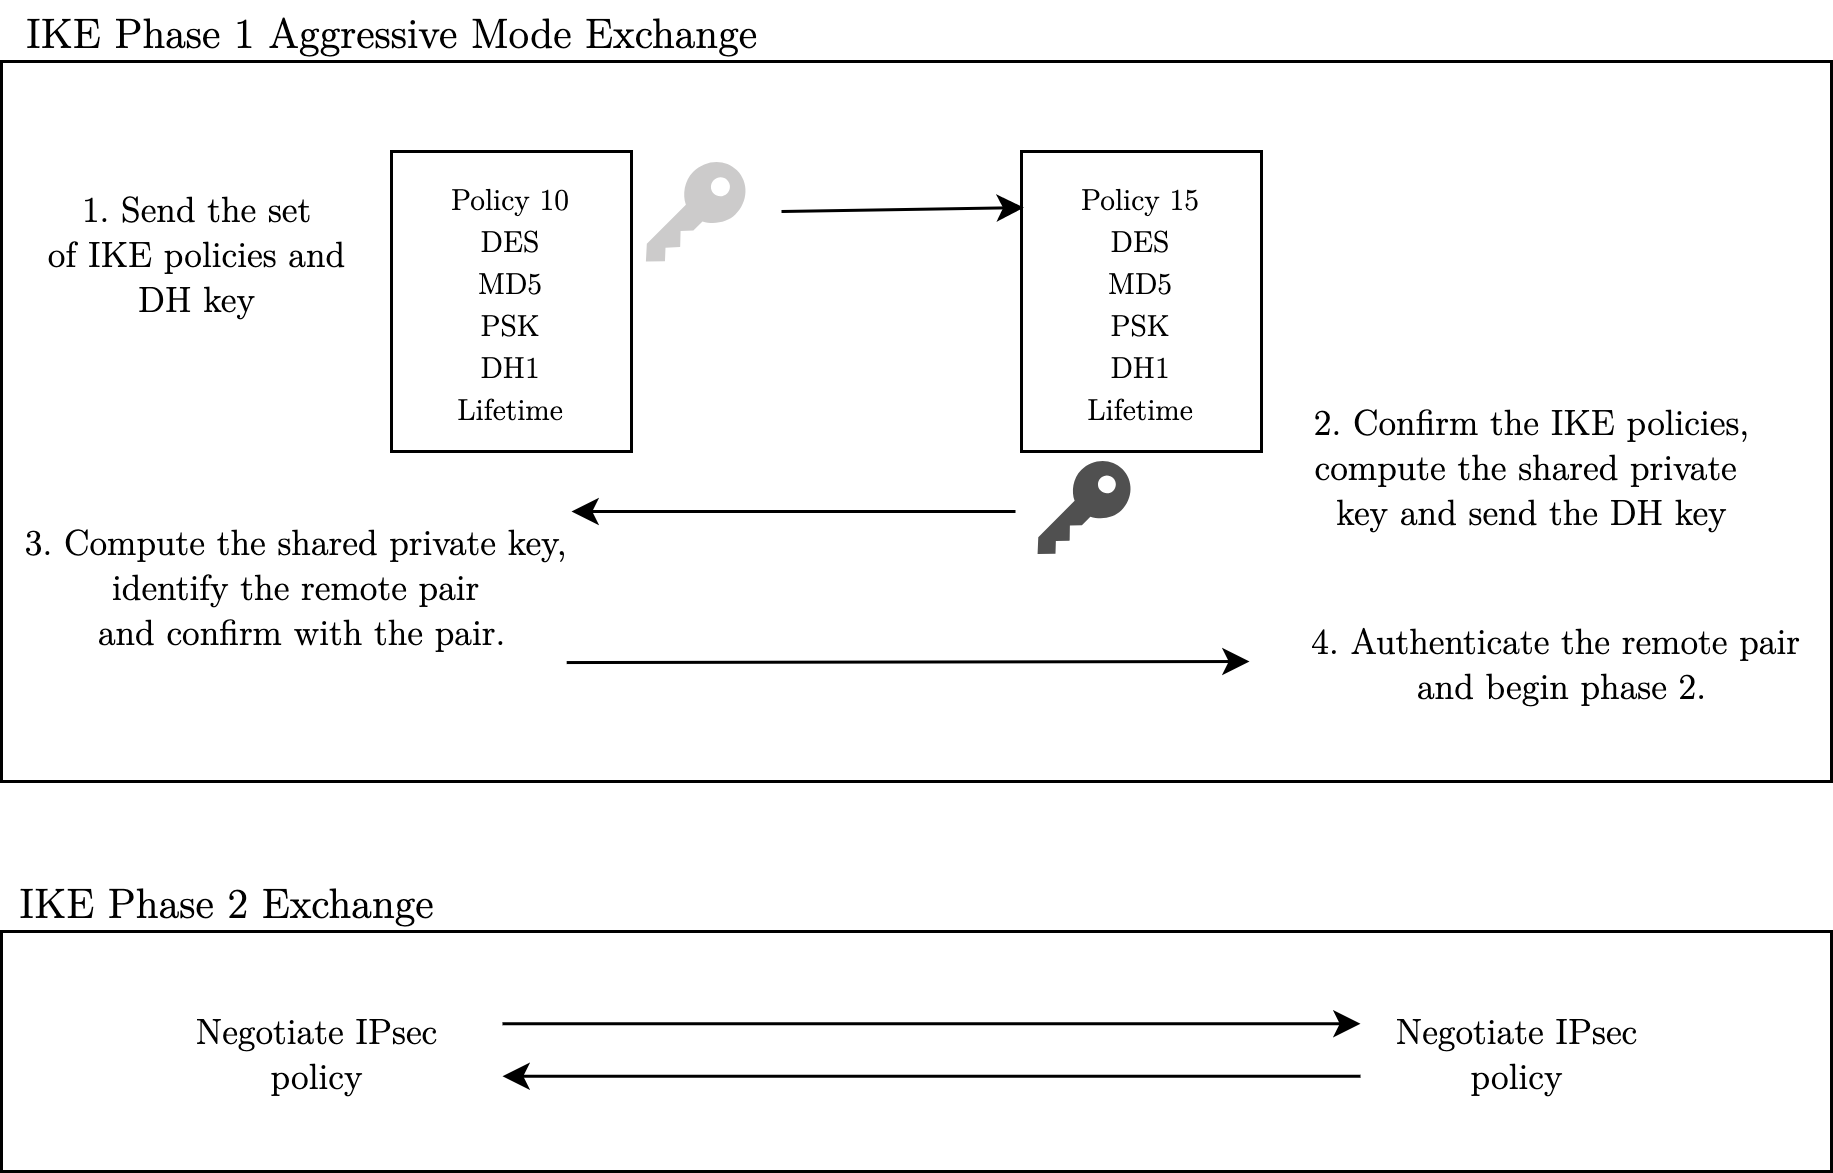
\includegraphics [scale=0.19] {aggressive.png}
	\caption{IKE: Phase 1 (Aggressive Mode) and Phase 2}
\end{figure}

\break

Finally in the following figure we can see the different algorithms used in order to establish a secure communication between two (or more) parties via IPsec implementation:

\begin{figure}[H]
	\centering
	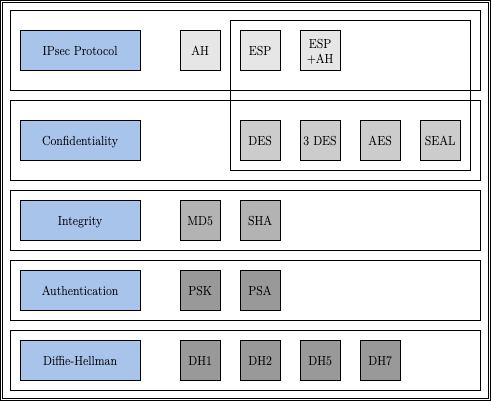
\includegraphics [scale=0.175] {summary.png}
	\caption{Algorithms}
\end{figure}
\section{Lightweight IPsec}
\chapter{CoAP: Constrained Application Protocol}
\section{Definition}
\subsection{Messaging Model}
\subsection{Request/Response Model}
\section{Message Format}
\section{Message Transmission}
\section{Securing CoAP}
\subsection{DTLS: Datagram Transport Layer Security}
\subsection{Key Management}
\chapter{Test - Setup}
\chapter{Test - Analysis}
\chapter{Conclusion}
\chapter{Discussion}

\end{document}
